\documentclass[11pt]{article}

\usepackage{acl}
\usepackage{pdfpages}
\usepackage{hyperref}
\usepackage{fancyvrb}

% Standard package includes
\usepackage{times}
\usepackage{latexsym}

% For proper rendering and hyphenation of words containing Latin characters (including in bib files)
\usepackage[T1]{fontenc}
\usepackage[ngerman]{babel}

% This assumes your files are encoded as UTF8
\usepackage[utf8]{inputenc}

% This is not strictly necessary, and may be commented out,
% but it will improve the layout of the manuscript,
% and will typically save some space.
\usepackage{microtype}

\title{Unicorn: Reasoning about Configurable System Performance through the Lens of Causality \\[16px] \normalfont{Reproduktion und Evaluation}}

\author{
  Alexander Vödisch \\
  \texttt{av21vupu@studserv.uni-leipzig.de} \\
}

\begin{document}

\maketitle

\begin{abstract}
In dieser Ausarbeitung werden die Ergebnisse von [ref] repliziert und evaluiert.
\end{abstract}

\section{Einführung}

Moderne Computersysteme sind oft aus einer Vielzahl von konfigurierbaren Komponenten aufgebaut, deren Zusammensetzung kritisch für die Systemperformance ist.\footnote{Unter (System-)Performance werden alle Leistungsmerkmale eines Systems wie beispielsweise Durchsatz und Energieverbrauch zusammengefasst.} Da die optimale Konfiguration dieser Komponenten hardwareabhängig sein kann und insbesondere in Kombination zu Pipelines der Konfigurationsraum exponentiell wachsen kann, sind spezielle Algorithmen notwendig, um Nutzer solcher Systeme bei der Definition möglichst optimaler Konfigurationen zu unterstützen.

Das Ziel von \textsc{Unicorn} ist es, für konfigurierbare Systeme die optimalen Konfigurationen bezüglich eines vom Nutzer definierten Merkmals (z.\,B. Leistung, Energieverbrauch, Inferenzzeit) zu finden und im Zuge dessen einen kausalen Graphen zu generieren, der als Modell auch auf bisher unbekannte Harware übertragen werden kann.

Im Gegensatz zu Modellen, die beispielsweise auf Regression basieren und lediglich den Einfluss individueller Konfigurationsoptionen messen, bietet \textsc{Unicorn} den Vorteil, dass nicht die Korrelation von Konfigurationsoptionen zur Vorhersage von guten Konfigurationen, sondern die kausalen Zusammenhänge der einzelnen Optionen für die Entwicklung des Modells genutzt werden. Dadurch kann das Modell auch in unbekannten Environments genutzt werden, wo korrelationsbasierte Performance-Influence-Modelle oft nur unzuverlässige Vorhersagen treffen.

\section{Funktionsweise}

\begin{figure}[tp!]
  \centering
  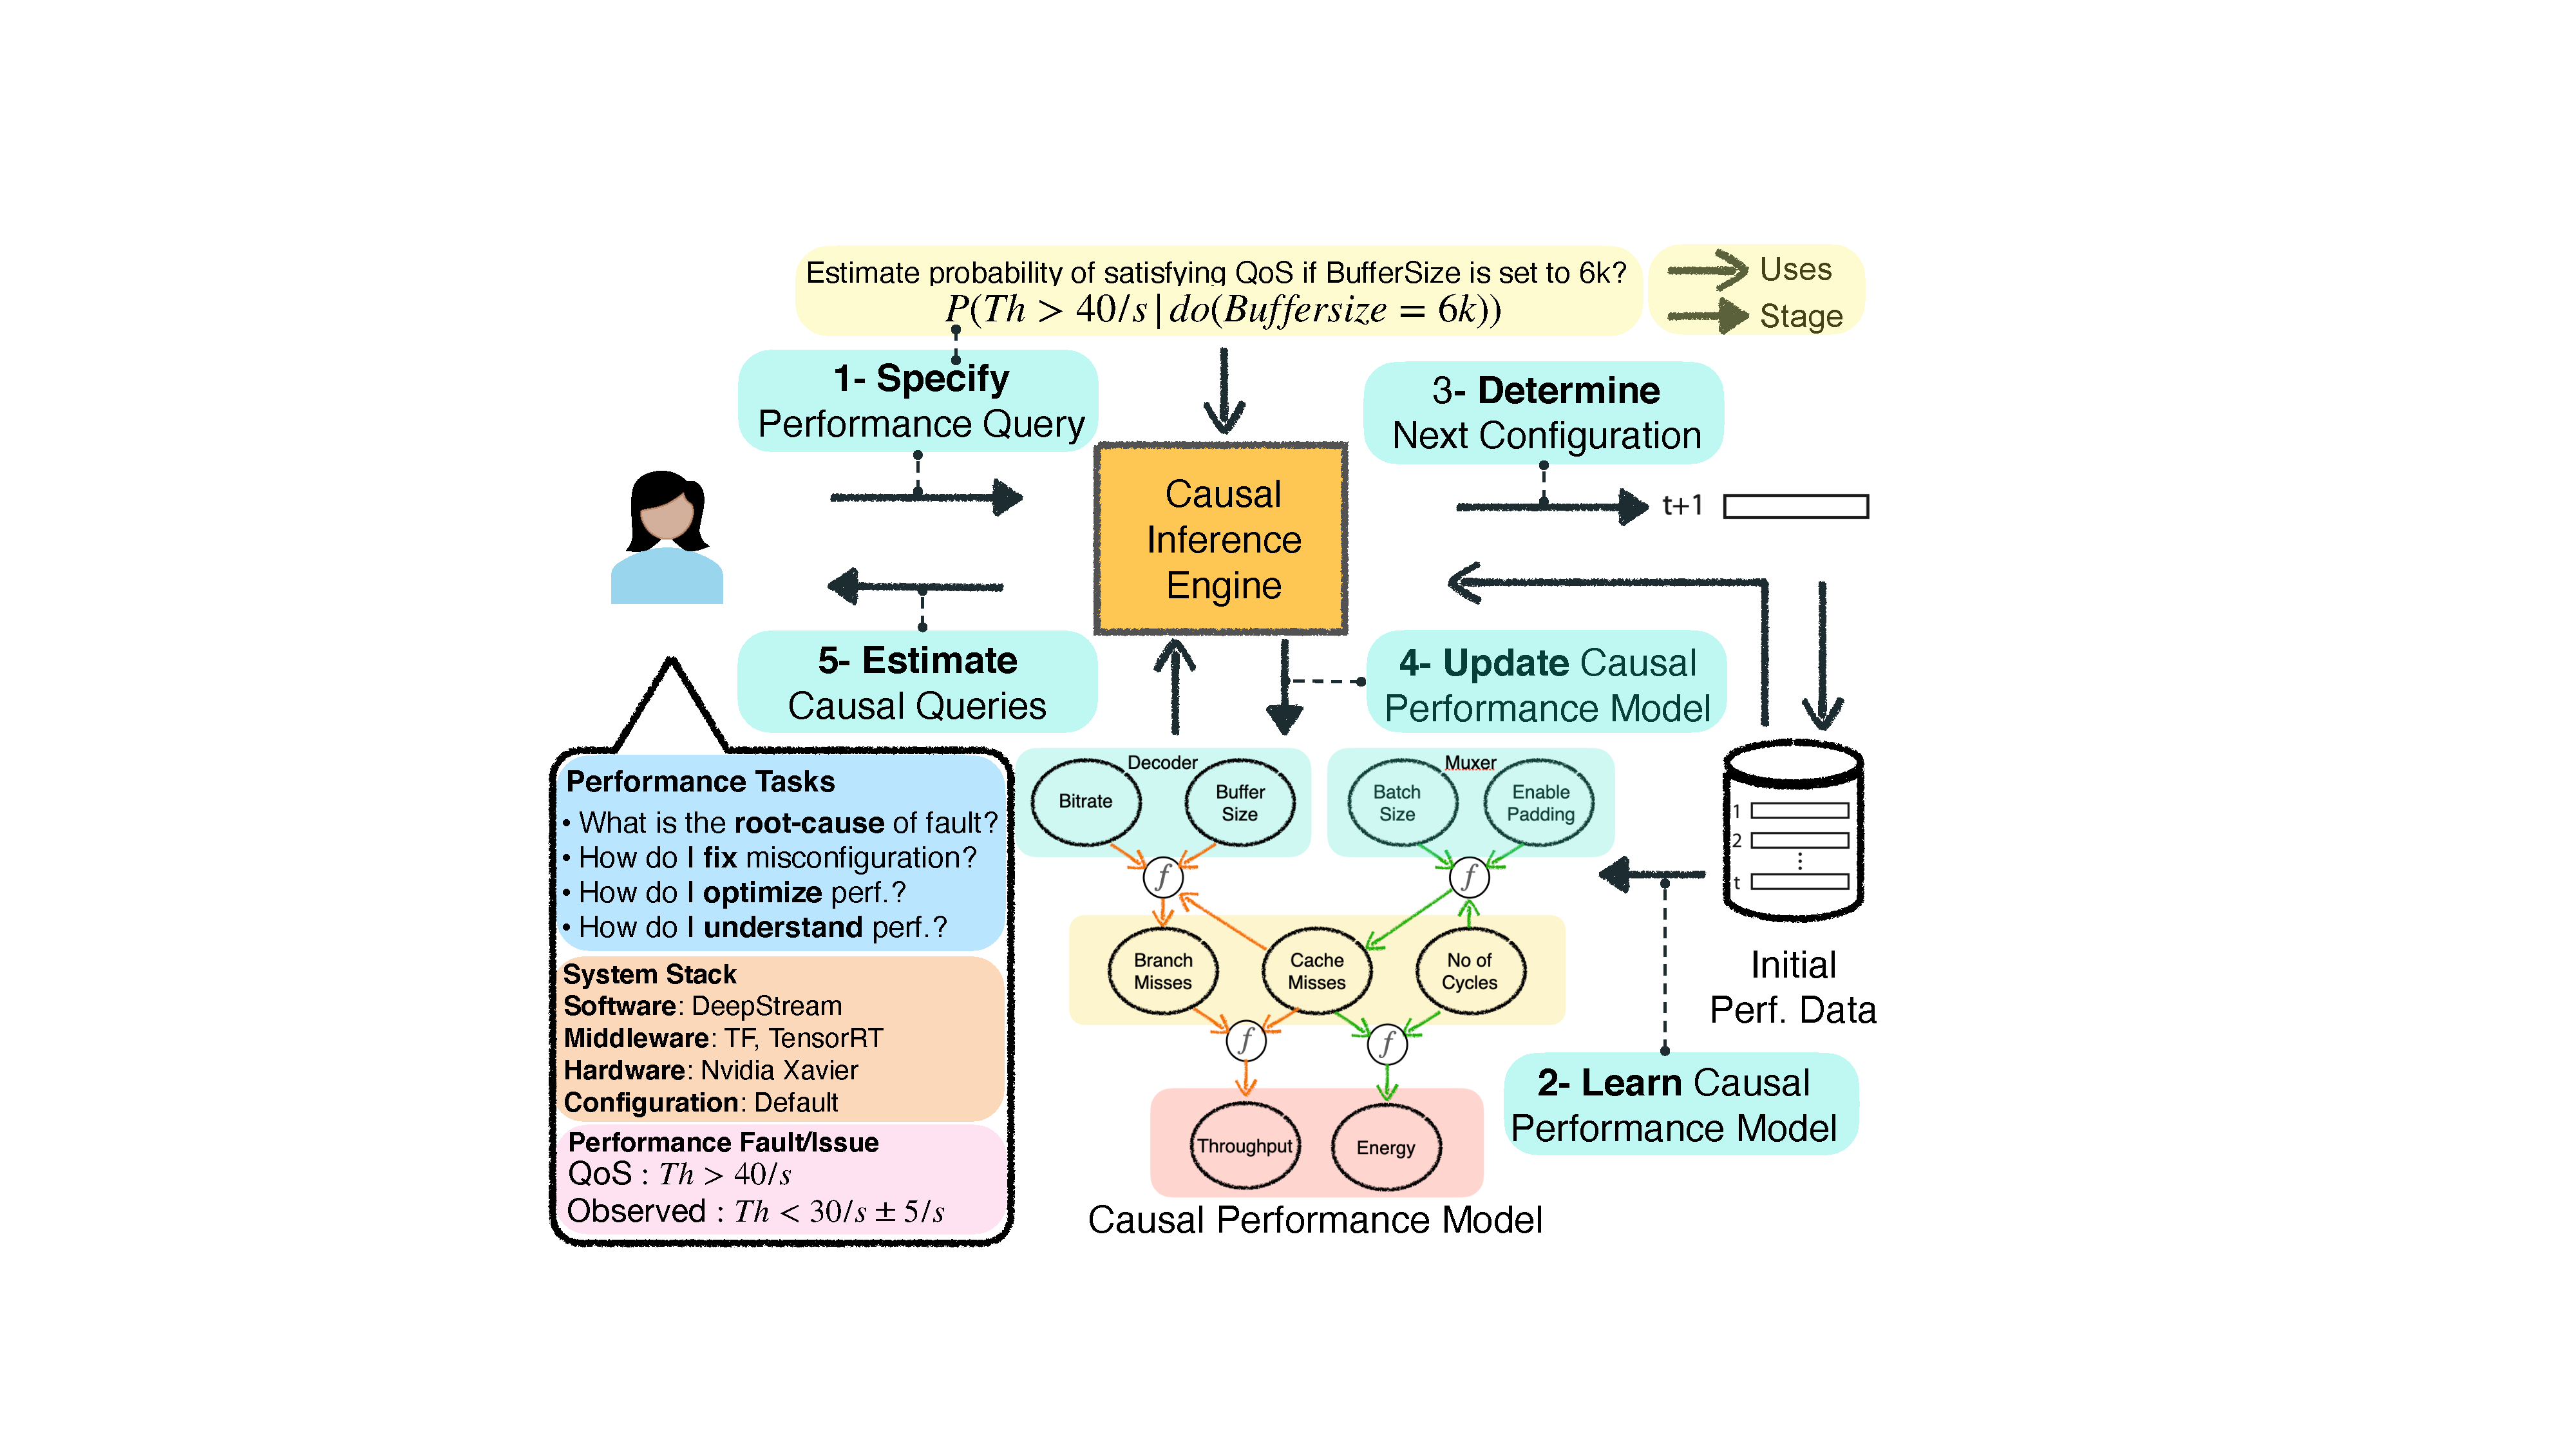
\includegraphics[width=\linewidth]{./img/UnicornOverview.pdf}
  \caption{Arbeitsweise von Unicorn.}

  \label{}
\end{figure}

\textsc{Unicorn} ermöglicht sowohl das Debuggen als auch auch das Optimieren von Systemkonfigurationen. Hierzu definieren die Autoren ein kausales Modell das auf probabilistischen graphischen Modellen basiert. Diese kausalen Graphen bestehen aus

\begin{itemize}
  \itemsep0em
  \item Performance-Variablen als Knoten für mögliche Konfigurationsparameter (z.\,B. \texttt{Birate}, \texttt{Buffer Size} oder \texttt{Batch Size}),
  \item funktionalen Knoten, die funktionale Abhängigkeiten zwischen den Performance-Variablen modellieren,
  \item kausalen Verbindungen zwischen den Performance-Variablen und den funktionalen Knoten und
  \item Nebenbedingungen, um notwendige Einschränkungen bei der Modellbildung zu definieren (z.\,B. dürfen \texttt{Cache Misses} nur positive ganzzahlige Werte annehmen).
\end{itemize}

\begin{figure}[tp!]
  \centering
  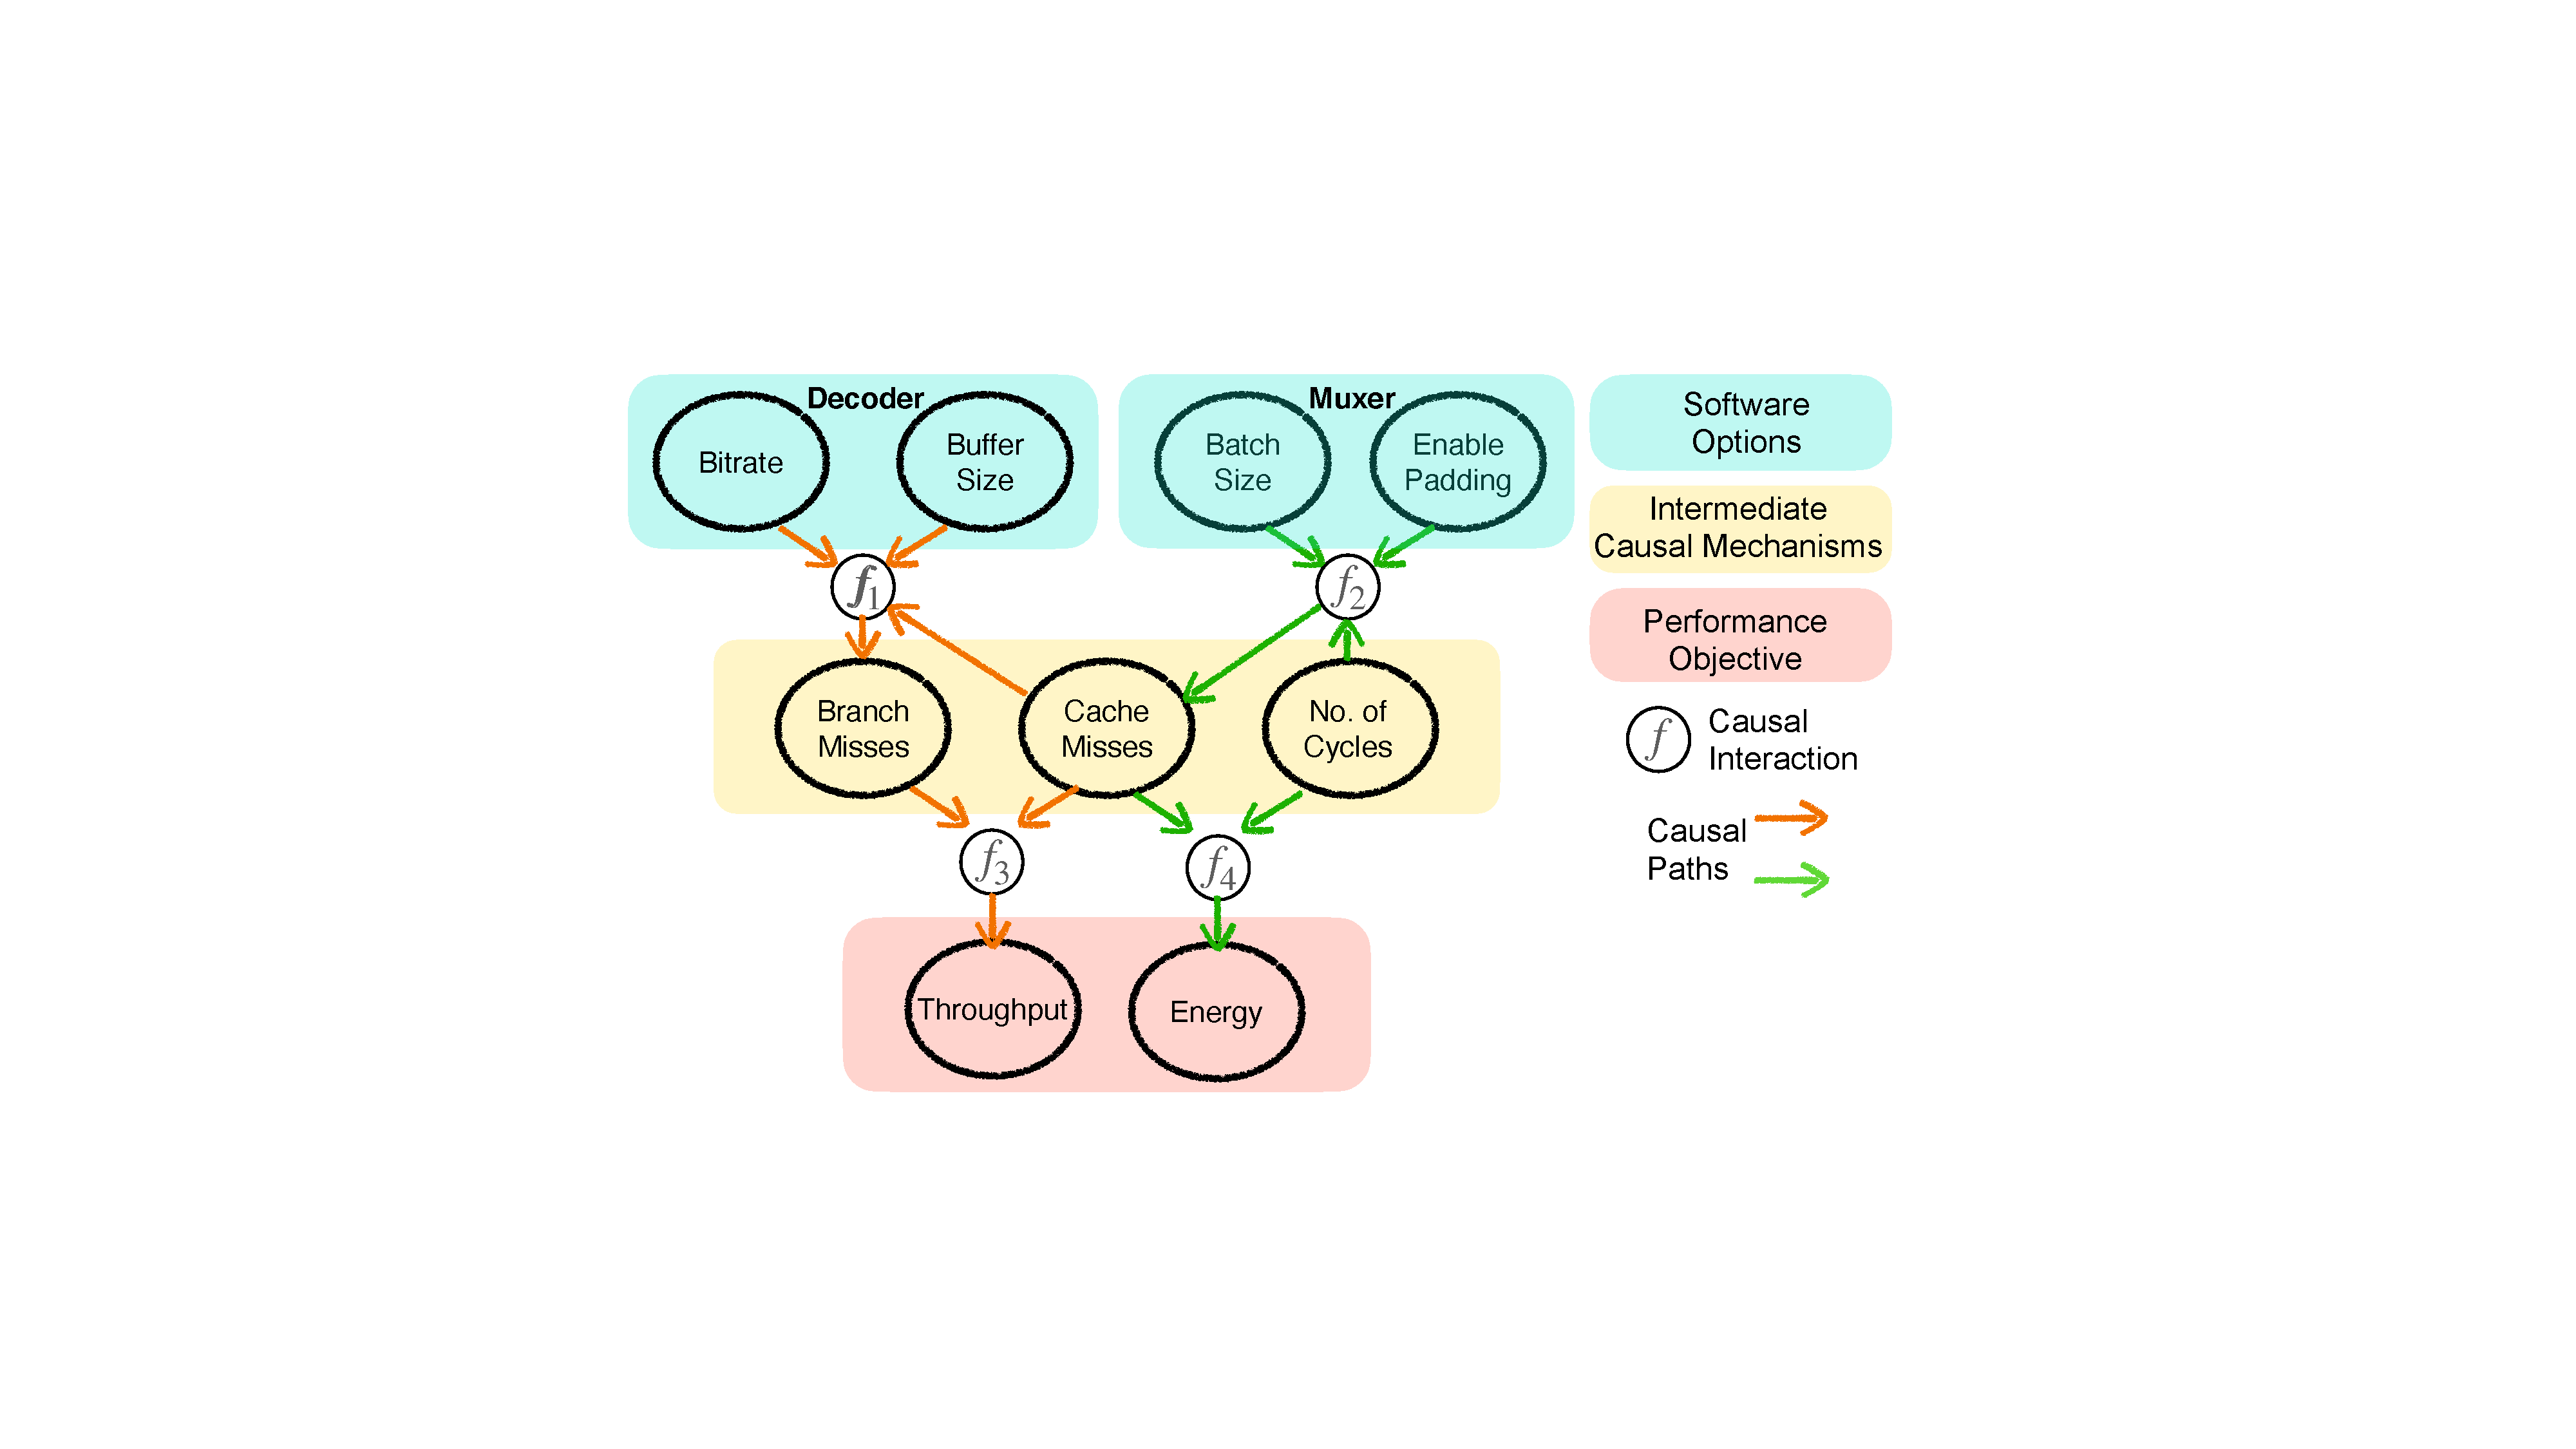
\includegraphics[width=\linewidth]{./img/CausalModelExample.pdf}
  \caption{Grundlegende Struktur des kausalen Graphen am Beispiel von Deepsteam, einer hochkonfigurierbaren Video-Analyse-Pipeline. Die Performance-Variablen sindd über funktionale Knoten miteinander Verbunden. Die Ausrichtung der Pfeile gibt an, zwischen welchen Performance-Variablen ein kausaler Zusammenhang besteht.}

  \label{}
\end{figure}

\textsc{Unicorn} arbeitet in 5 Schritten:
\begin{enumerate}
  \itemsep0em
  \item Spezifikation der Optimierungsanforderung als Klartext durch den Nutzer
  \item Lernen des kausalen Modells mittels vordefinierter Anzahl an Musterkonfigurationen: Hierfür wird der \textit{Fast Causal Inference}-Algorithmus genutzt, um Kanten von dem zunächst vollständigem probabilistischen Graphen entsprechend der Nebenbedingungen zu entfernen und ungerichtete Kanten entsprechend der kausalen Einflüsse der Performance-Variablen auszurichten.
  \item Bestimmung der Folgekonfiguration und Messen der Systemperformance: Für die Folgekonfiguration werden diejenigen Performance-Variablen angepasst, die kausal am stärksten Zusammenhängen, um den Lernprozess zu beschleunigen (\textit{Active Learning}).
  \item Inkrementelles Update des kausalen Modells
  \item Wiederholung der Schritte 3 und 4 bis ein vordefiniertes Limit (z.\,B. Laufzeit) überschritten wurde und anschließend Ausgabe
\end{enumerate}

\begin{figure}[tp!]
  \centering
  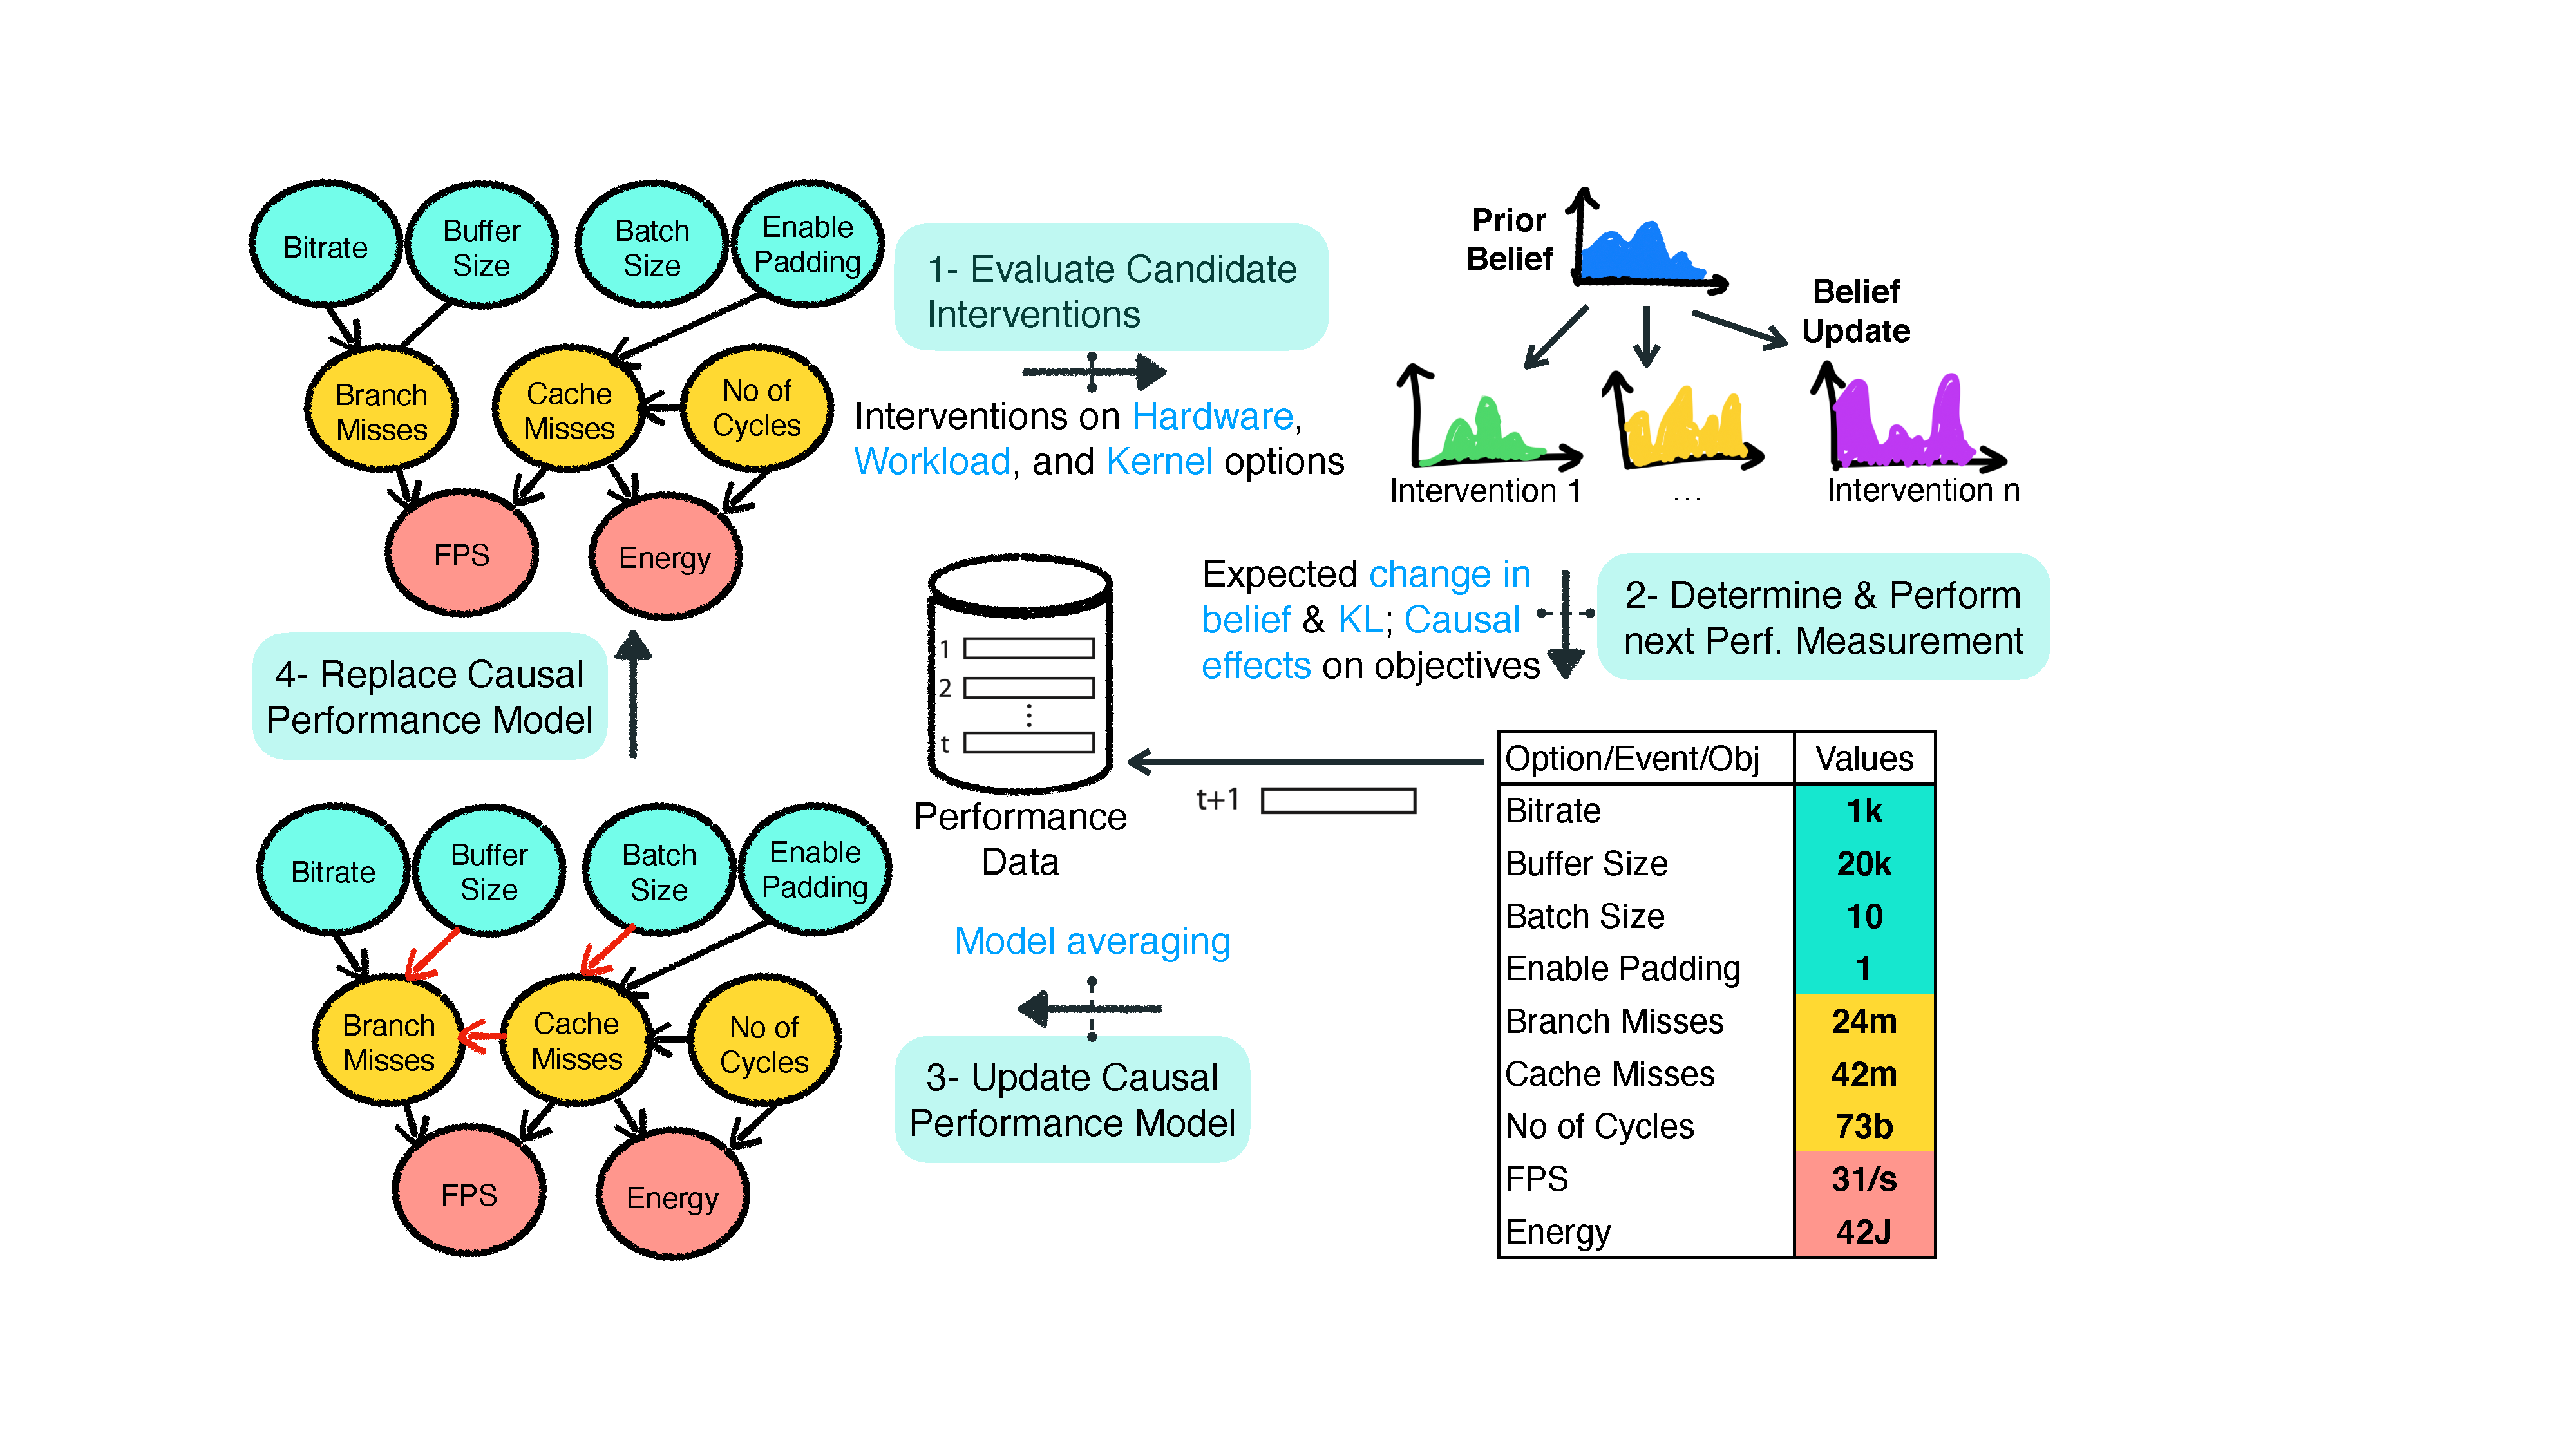
\includegraphics[width=\linewidth]{./img/Causal-Model-Update.pdf}
  \caption{Update des kausalen Modells. Zunächst wird werden die Einflüsse der vorigen Konfigurationsänderungen abgeleitet. Anschließend wird die Konfiguration entsprechend den erwarteten Auswirkungen auf die vom Nutzer gestellten Performance-Objectives angeglichen. Daraufhin wird der kausale Graph angepasst und das Modell aktualisiert.}

  \label{}
\end{figure}

\section{Fallbeispiele}

In dieser Ausarbeitung werden die Ergebnisse der Evaluation von \textsc{Unicorn} anhand der Fallbeispiele aus dem Originalpaper repliziert.

\textsc{Unicorn} kann im Online- oder Offline-Modus betrieben werden. Im Online-Modus werden die Performance-Metriken direkt auf der zugrundeliegenden Hardware ausgeführt. Der Offline-Modus erlaubt die Reproduktion auf beliebiger Hardware. Da uns die im Paper genutzte Hardware nicht zur Verfügung steht, werden lediglich die Ergebnisse der Offline-Evaluation repliziert.

Die Autoren stellen den Quellcode als Python-Bibliothek auf GitHub zur Verfügung.\footnote{\href{https://github.com/softsys4ai/unicorn}{https://github.com/softsys4ai/unicorn}} Eine Dokumentation sowie eine ausführliche Anweisungen zur Replikation der Ergebnisse sind im Repository angehängt. Entsprechend den Anweisungen wurde Docker in Version \texttt{20.10.16} auf den Testsystemen installiert.

Bis auf ein fehlendes Paket, das zur Ausführung auf unseren Systemen notwendig war, konnten die Tests ohne Probleme ausgeführt werden. \textsc{Unicorn} erzeugt nach dem Testläufen mit \texttt{matplotlib} Graphen. In manchen Fällen konnten die Graphen nicht gespeichert werden, was jedoch nicht auf die eigentlichen Tests und deren Ergebnisse zurückzuführen ist.

Die Replikation findet auf zwei Testsystemen statt:\footnote{Die Testsysteme werden im Folgenden kurz als \texttt{Win} und \texttt{Mac} bezeichnet.}
\begin{itemize}
  \itemsep0em
  \item \texttt{Windows 10 21H2} mit \texttt{Intel Core i7-8700K CPU @ 12x3.50 GHz} und \texttt{32GB DDR4 RAM @ 3280Mhz}
  \item \texttt{MacOS Monterey 12.4} mit \texttt{Apple M1 CPU @ 4x3.20 GHz} und \texttt{16 GB LPDDR-DDR4X RAM @ 4266 Mhz}
\end{itemize}
Den Docker-Containern werden je 4 CPU-Kerne und 8 GB Arbeitsspeicher zur Verfügung gestellt.

Das System der Autoren im Offline-Mode verwendet als Prozessor \texttt{Intel Core i7-8700 CPU @ 12x3.20 GHz} und besitzt \texttt{31.2 GB} an Arbeitsspeicher, die zugrundeliegende Hardware ist zu unserem ersten System sehr ähnlich. Als Betriebssystem verwenden die Autoren jedoch \texttt{Ubuntu 18.04}.

Wir werden im Folgenden die Resultate der drei Kernbehauptungen des Originalpapers reproduzieren:

\begin{itemize}
  \itemsep0em
  \item \textsc{Unicorn} kann für das Aufsprüren der Ursachen von nicht-funktionalen Fehlern (Latenz, Energieverbrauch) genutzt werden.
  \item \textsc{Unicorn} kann als Werzeug bei der Durchführung von Performanceoptimierungen unterstützen.
  \item \textsc{Unicorn} ist effizient, auch wenn sich das Einsatzenvironment ändert.
\end{itemize}

\section{Replikation der Ergebnisse}

Für die Reproduktion der Ergebnisse werden die Anweisungen der Dokumentation in \texttt{artifact/REPRODUCE.md} genutzt. Leider konnten bei einigen der Experimente die von \textsc{Unicorn} ausgegeben Graphen nicht gespeichert werden, so dass der zeitliche Verlauf beispielsweise bei der Optimierung nicht ersichtlich ist.

\subsection{Erkennung der Ursachen für hohen Energieverbrauch}\label{sec:1}

In diesem Experiment soll die Ursache für den hohen Energieverbrauch ermittelt und eine Lösung hierfür gefunden werden.

\begin{figure}[tp!]
  \centering
  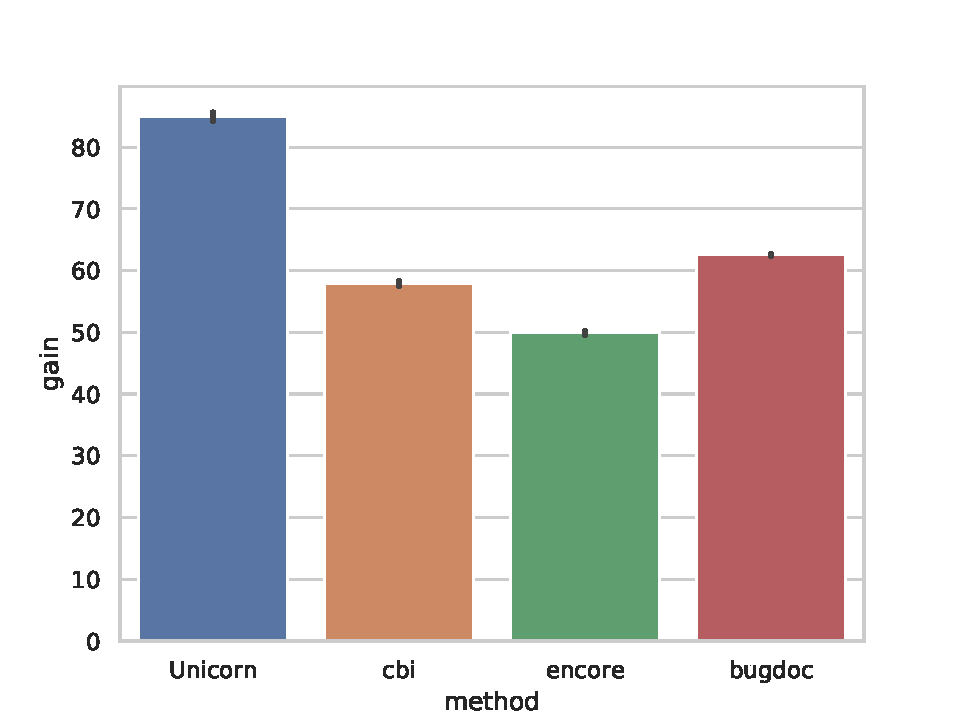
\includegraphics[width=\linewidth]{./img/win_debug_gain.pdf}
  \caption{Verbesserung des Energieverbrauchs gegenüber Standardkonfiguration bei Einsatz von \textsc{Unicorn}, CBI, \textsc{EnCore} und \textsc{BugDoc}. Die Ergebnisse sind für \texttt{Win} und \texttt{Mac} identisch.}

  \label{fig:1}
\end{figure}

\begin{figure}[tp!]
  \centering
  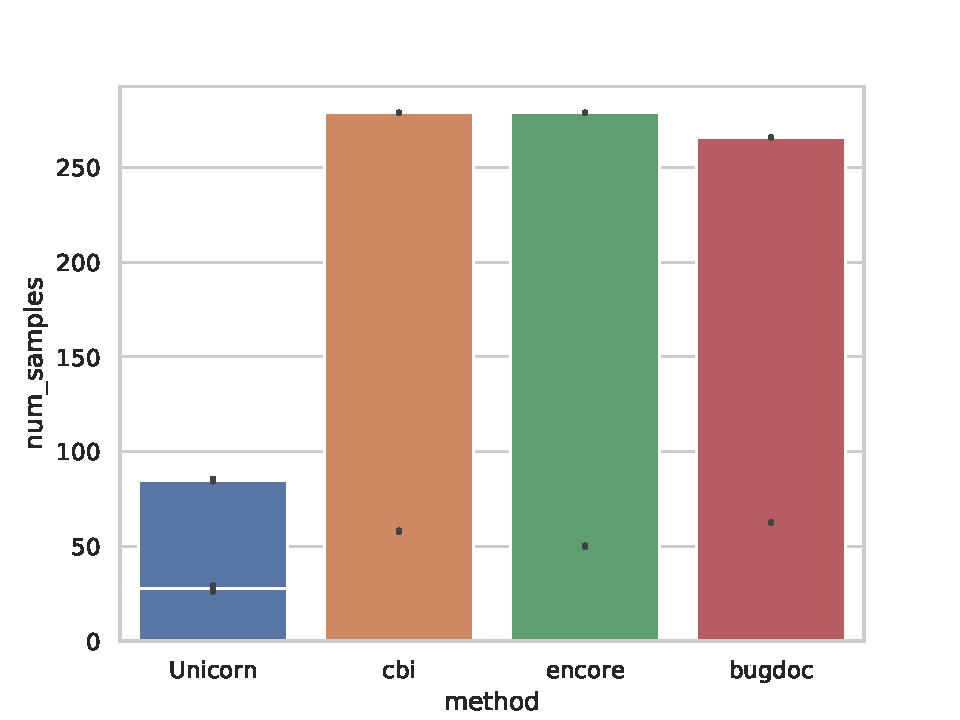
\includegraphics[width=\linewidth]{./img/win_debug_num_samples.pdf}
  \caption{Notwendige Anzahl an Samples}

  \label{fig:3}
\end{figure}

\begin{figure*}
  \centering
    \begin{Verbatim}[fontsize=\small,samepage=true]
      +++++++++++++++++++++++++++++++++++++++++++++BUG+++++++++++++++++++FIX
      memory_growth                                0.5            5.0000e-01
      logical_devices                              1.0            1.0000e+00
      core_freq                              1651200.0            1.5744e+06
      gpu_freq                               1651200.0            1.6512e+06
      emc_freq                             800000000.0            2.1330e+09
      num_cores                                    2.0            2.0000e+00
      scheduler.policy                             1.0            1.0000e+00
      vm.swappiness                              100.0            1.0000e+02
      vm.vfs_cache_pressure                      500.0            5.0000e+02
      vm.dirty_background_ratio                   80.0            8.0000e+01
      vm.drop_caches                               3.0            3.0000e+00
      vm.nr_hugepages                              1.0            1.0000e+00
      vm.overcommit_ratio                         50.0            5.0000e+01
      vm.overcommit_memory                         1.0            1.0000e+00
      vm.overcommit_hugepages                      2.0            2.0000e+00
      kernel.sched_child_runs_first                0.0            0.0000e+00
      kernel.sched_rt_runtime_us              500000.0            5.0000e+05
      vm.dirty_bytes                              30.0            3.0000e+01
      vm.dirty_background_bytes                   60.0            6.0000e+01
      vm.dirty_ratio                               5.0            5.0000e+00
      swap_memory                                  1.0            1.0000e+00
      kernel.max_pids                          32768.0            6.5536e+04
      kernel.sched_latency_ns               24000000.0            2.4000e+07
      kernel.sched_nr_migrate                    256.0            2.5600e+02
      kernel.cpu_time_max_percent                 50.0            5.0000e+01
      kernel.sched_time_avg_ms                  1000.0            1.0000e+03
    \end{Verbatim}
    \caption{Ausgabe einer Iteration von \textsc{Unicorn} bei der Optimierung der Inferenzzeit. In der Mittleren Spalte befinden sich die Werte der fehlerhaften Konfiguration. Rechts befindet sich die von \textsc{Unicorn} vorgeschlagene Konfiguration.}

    \label{fig:2}
\end{figure*}

\begin{figure*}[tp!]
  \centering
  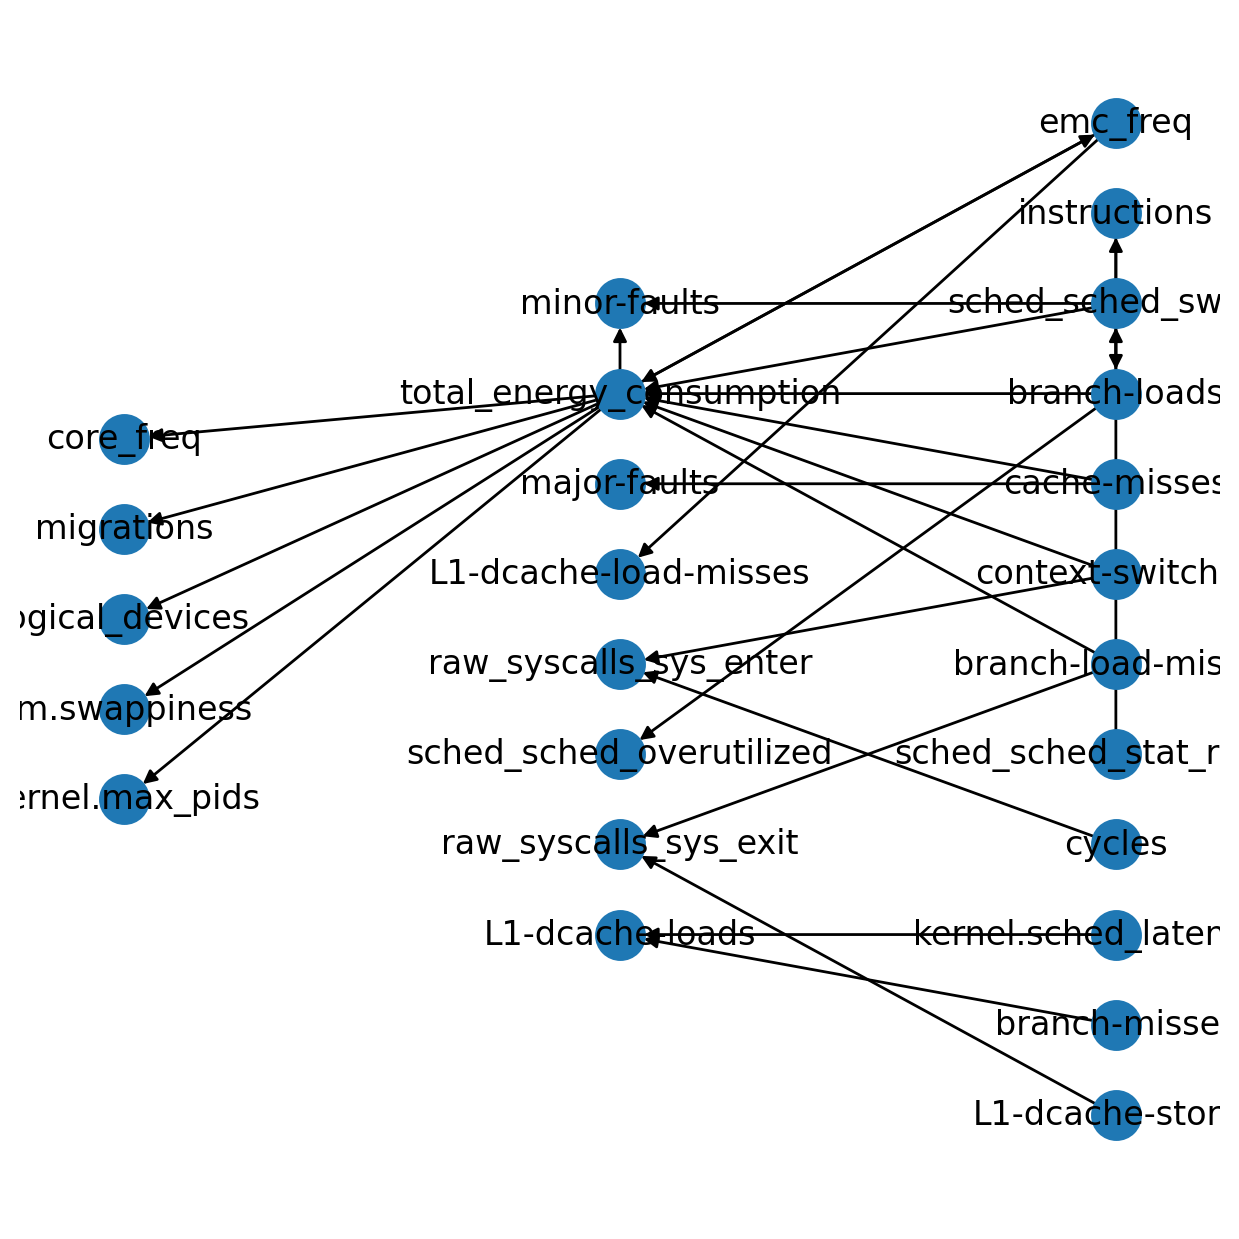
\includegraphics[width=\linewidth]{./img/causal_graph.png}
  \caption{Von \textsc{Unicorn} gelernter kausaler Graph des Experiments aus Abschnitt \ref{sec:1}.}

  \label{fig:2}
\end{figure*}

Wie in Abbildung \ref{fig:1} zu sehen ist, entspricht der \textit{Gain}, d.\,h. der Zuwachs an Performance und somit die Verringerung des Energieverbrauchs, bei unseren Experimenten den Ergebnissen der Autoren. Der in Abbildung \ref{fig:2} gezeigte kausale Graph gibt Aufschluss darüber, welche Konfigurationsparameter Einfluss auf den Energieverbrauch haben. Die genauen Werte sind im von \textsc{Unicorn} ausgegeben Log zu sehen:

Wie zu erwarten schlägt \textsc{Unicorn} Änderungen bei den Frequenzen (\texttt{core\_freq}, \texttt{gpu\_freq} und \texttt{emc\_freq}) vor. Die Ergebnisse der Autoren konnten in diesem Fall sehr gut repliziert werden.

\subsection{Optimierung der Inferenzzeit}

In diesem Experiment wird die minimale Latenz, d.\,h. die Inferenzzeit, optimiert.

Das lokale Optimum von 12 Sekunden Inferenzzeit erreicht \textsc{Unicorn} bereits nach 69 Iterationen. Auf \texttt{Win} benötigt es dafür ca. 280 Minuten, auf \texttt{Mac} benötigt es 70 Minuten, die nötige Laufzeit von Unicorn auf \texttt{Win} war also sehr viel länger war als auf \texttt{Mac} und damit deutlich länger als in der Dokumentation angegeben (ca. 90 Minuten). Grundsätzlich ist hierbei nicht davon auszugehen, dass die zugrundeliegende Hardware dafür verantwortlich ist, da die Autoren bei ihren Experimenten die gleiche CPU verwendet haben. Möglicherweise ist eine Systemkonfiguration außerhalb des Containers, in dem die Berechnungen stattfanden, dafür verantwortlich (Docker von \texttt{Win} basiert auf WSL2 was beim Testsystem der Autoren, das auf Ubuntu basiert, nicht der Fall ist).

Auch hier stimmen die Resultate mit den Ergebnissen im Paper überein. \textsc{Unicorn} erreicht das lokale Optimum bereits nach 69 Iterationen und damit schneller als SMAC. Andererseits ist das von \textsc{Unicorn} gefundene Optimum um 8 Sekunden besser als das von SMAC.

Beim Vergleich der Laufzeit von SMAC und \textsc{Unicorn} konnten wir sehr große Unterschiede feststellen. Obwohl die Laufzeit auf \texttt{Mac} wie im Paper beschrieben bis zu 90 Minuten dauern kann (in unserem Fall waren es ca. 70 Minuten), war SMAC mit einer Laufzeit von nur 50 Sekunden auf \texttt{Win} und 23 Sekunden auf \texttt{Mac} um ein Vielfaches schneller. Für die Optimierung der Inferenzzeit sollte also die lange Laufzeit von \textsc{Unicorn} berücksichtigt werden. Wird die Optimierung häufig ausgeführt ist SMAC mit seiner Geringeren Laufzeit vorzuziehen.

\subsection{Änderung der Hardware}

In diesem Experiment wird die Übertragbarkeit des von \textsc{Unicorn} gelernten Modells untersucht.

Für den Vergleich der Performance auf unterschiedlicher Hardware werden von den Autoren drei Fälle untersucht: Im ersten Fall (\textit{Reuse}) wird das Modell mit der initialen Hardwarekonfiguration trainiert und anschließend der Gain auf der neuen Hardware ermittelt, ohne dabei das Modell neu zu trainieren oder neue Samples zur verfügung zu stellen. Im zweiten Fall (\textit{Reuse+25}) wird das Modell auf die neue Hardware übertragen und mit 25 neuen Samples an die neue Hardwarekonfiguration angepasst. Wie weiter oben erwähnt benötigt \textsc{Unicorn} lediglich etwa 25 Samples um gute Ergebnisse zu erziehlen. Durch diese geringe Anzahl an Samples sollten somit die Performancezuwächse gegenüber dem \textit{Reuse}-Fall verbessert werden, ohne dabei die gesamte Laufzeit für ein vollständiges Retraining zu benötigen. Im dritten Fall wird das Modell nicht übertragen und somit komplett neu trainiert.

Es ist zu erwarten, dass zwar der Gain von Fall 1 bis 3 zunimmt, gleichzeitig aber auch die Laufzeit.

Wir konnten die Ergebnisse der Autoren genau reproduzieren und konnten keine signifikanten Abweichungen bei den benötigen Laufzeiten feststellen. Wie vermutet ist der Gain bei \textit{Reuse} des Modells am geringsten mit ca. 68 \%, benötigt dabei allerdings kein Retraining und somit existiert keine Trainingszeit. Im Vergleich zum \textit{Reuse+25}, bei dem das Modell ein Gain von etwa 80 \% erzielt hat, benötigt \textsc{Unicorn} etwa 10 Minuten. Der Performancezuwachs zwischen \textit{Reuse} und \textit{Reuse+25} liegt somit bei ca. 12 \%. Bei vollständigem Neutrainieren des Modells benötigt Unicorn mit 20 Minten am längsten, erzielt aber einen Gain von 82 \%, also etwa 2 \% mehr als im zweiten Fall mit nur 25 Samples. Der Performancezuwachs ist also zwischen diesen Fällen gering, was zeigt, dass \textsc{Unicorn} einerseits bereits mit keinen oder wenigen Samples gute Performaancezunahmen auf neuer Hardware erreicht, andererseits für noch bessere Ergebnisse nur wenige Samples benötigt.

\begin{figure*}[!htbp]
  \centering
  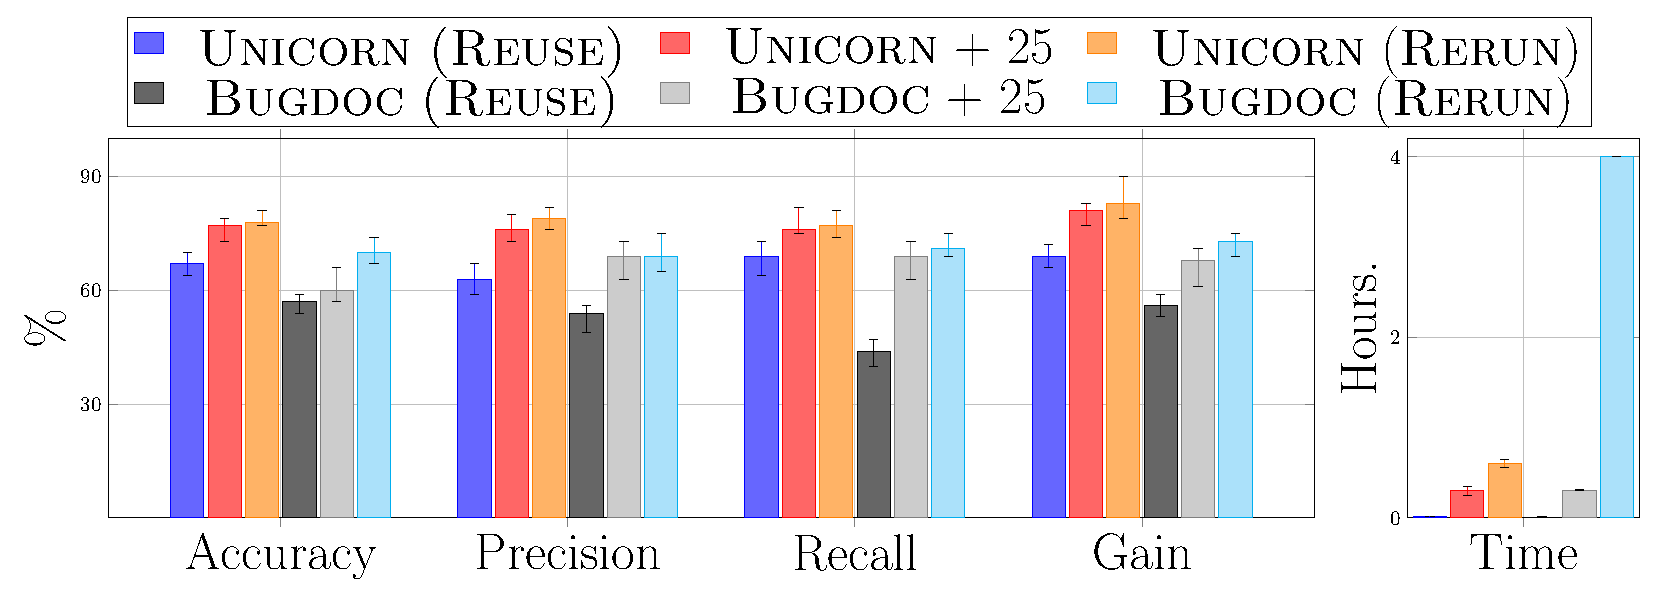
\includegraphics[width=\linewidth]{./img/barplot_multi_debug_orig.pdf}
  \caption{Vergleich der Performancemetriken von \textsc{Unicorn} mit Bugdoc. In allen Fällen hat \textsc{Uniform} bessere Werte als Bugdoc erziehlt. Für das Retraining der Modelle mit 25 Samples benötigen beide Algorithmen etwa gleich lang.}

  \label{fig:2}
\end{figure*}

\section*{Fazit}

\textsc{Unicorn} ermöglicht das Optimieren von hochkonfigurierbaren System hinsichtlich Energieverbrauch undd Inferenzzeit. Dabei sind die von \textsc{Unicorn} gefundenen Konfigurationen, wie von den Autoren empirisch gezeigt und von uns bestätigt, fast immer besser als die von gängigen Modellen wie Bugdoc oder SMAC, benötigt jedoch wesentlich länger um diese Ergebnisse zu erzielen. Als Vorteil von \textsc{Unicorn} ist die geringe Anzahl an benötigten Samples und die guten Resultate bei der Übertragung des Modells auf neue Hardware zu nennen.

Bei der Reproduktion der Resultate des Originalpapers ist die gute Dokumentation hervorzuheben, wodurch die Replikation der Ergebnisse -- bis auf wenige unkritische Probleme bei der Ausführung von Windows als Betriebssystem -- sehr einfach war. Unsere Ergebnisse bei der Optimierung entsprechen denen im Originalpaper. Lediglich die Laufzeit auf Windows war in wenigen Ausnahmen wesentlich länger als von den Autoren angegeben.

\end{document}
